  \begin{theorem}[O ciągu stopni w grafie]
      Niech liczby $(d_1, d_2, d_3, \dots, d_n)$ są takie, że $(d_1 \leq d_2 \leq d_3 \leq \dots d_n)$. Przez $(d_1', d_2', \dots, d_{n-1}')$ oznaczamy ciąg liczb taki, że: \begin{equation}
          d_i' = \begin{cases}
              d_i \hspace{5pt} \mathrm{, gdy } \hspace{5pt} i < n - d_n \\
              d_i-1 \hspace{5pt} \mathrm{, gdy } \hspace{5pt} i \geq n - d_n
          \end{cases}
      \end{equation}
      $(d_1 \leq d_2 \leq d_3 \leq \dots d_n)$ jest sekwencją grafową wtedy i tylko wtedy, gdy $(d_1', d_2', \dots, d_{n - 1}')$ jest sekwencją grafową. 
  \end{theorem}
  \begin{proof}
      To twierdzenie brzmi na początku totalnie randomowo, ale ma sens. Najlepiej chyba pokazać skąd to się wytrzasnęło, przeprowadzając dowód w drugą stronę (tzn. jeśli $(d_1' \dots)$ to poprawny ciąg, to $(d_1 \dots)$ to również poprawna sekwencja grafowa).

    No dobra, to powiedzmy że mamy poprawną sekwencję grafową $(d_1', \dots, d_{n-1}')$. Sekwencję z której ona powstała otrzymuję w ten sposób, że do grafu $G$ który jest reprezentowany przez poprawną sekwencję po prostu dorzucam jeden wierzchołek i ,,podłączam'' go do tylu ostatnich wierzchołków w sekwencji, żeby się ,,zgodziło'' (czyli do $d_n$). Jak się spojrzy na definicję sekwencji to powinno się to robić oczywiste dlaczego to działa.

    W drugą stronę jest to nieco mniej oczywiste.\\
    Rozważmy najpierw prosty przypadek: $d_n = n - 1$. Oznacza to, że ostatni wierzchołek jest podłączony do wszystkich pozostałych wierzchołków. Zatem jeśli go usuniemy, to dostaniemy po prostu graf, którego sekwencją stopni jest $\pars{d_1', d_2', \ldots, d_{n - 1}'}$, co widać z~definicji. Zatem w~tym przypadku wszystko się zgadza.\\
    Teraz rozważmy sytuację, w~której $d_n < n - 1$. Chcemy pokazać, że istnieje graf, którego sekwencją stopni jest $\pars{d_1', \ldots, d_{n - 1}'}$. W~tym celu pokażemy, że istnieje graf o~sekwencji $\pars{d_1, \ldots, d_n}$ taki, że ostatni wierzchołek jest podłączony do $d_n$ wierzchołków bezpośrednio przed nim. Wtedy zadziała identyczny trik z~odrzuceniem tego wierzchołka i~zmniejszeniem stopnia jego sąsiadom o~$1$, aby otrzymać elegancki graf o~sekwencji $\pars{d_1', \ldots, d_{n - 1}'}$. Udowodnimy to nie wprost: załóżmy, że tak, nie jest. Sformalizujmy to założenie. Rozważmy zbiór wszystkich grafów, które mają taką sekwencję stopni, jak nasz wyjściowy graf:
    
    \begin{equation*}
        \mathcal{G} = \left\{G : V\pars{G} = \left\{v_1, \ldots, v_n\right\} \land \forall_{i \in [n]}\deg_G\pars{v_i} = d_i\right\}
    \end{equation*}
    
    Zakładamy zatem, że dla każdego $G \in \mathcal{G}$ istnieje takie $i \in [n - d_n, n - 1]$, że $v_iv_n \not\in E\pars{G}$, tzn. każdy graf o~interesującej nas sekwencji wierzchołków ma ,,dziurę'' (nie-sąsiada) wśród $d_n$ wierzchołków bezpośrednio poprzedzających $v_n$.
    
    Możemy zatem zdefiniować fajną funkcję:
    
    \begin{gather*}
        j\colon \mathcal{G} \mapsto [n - d_n, n - 1]\\
        j\pars{G} = \max\left\{i \in [n - d_n, n - 1] : v_iv_n \not\in E\pars{G} \right\}
    \end{gather*}
    
    Intuicyjnie, funkcja $j$~wskazuje indeks najpóźniejszej ,,dziury'' w~danym grafie. Weźmy taki graf $G \in \mathcal{G}$, dla którego $j\pars{G}$ jest \emph{najmniejsze} możliwe (graf, który najpóźniejszą dziurę ma możliwie najwcześniej). Oczywiście wolno nam to zrobić, bo $\mathcal{G}$ jest zbiorem skończonym. Aby uprościć zapis, przyjmijmy $j = j\pars{G}$.
    
    \begin{figure}[H]
        \centering
        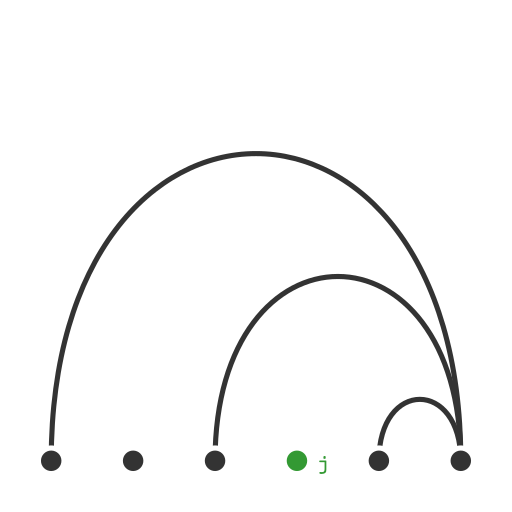
\includegraphics[width=0.3\textwidth]{images/two_holes.png}
        \caption{,,Dziury'' wśród $d_n$ wierzchołków poprzedzających $v_n$}
    \end{figure}
    
    Wiemy, że istnieje takie $k < j$, że $v_kv_n \in E\pars{G}$, bo inaczej wszyscy sąsiedzi $v_n$ byliby tuż przed nim i~nie byłoby ,,dziury''. Wiemy też, że $d_k \leq d_j$, bo mamy do czynienia z~sekwencją grafową. Ale to oznacza, że istnieje takie $s$, że $v_sv_j \in E\pars{G}$, ale $v_sv_k \not\in E\pars{G}$. Dlaczego? Ponieważ, gdyby tak nie było, to $v_k$ miałby krawędzie do wszystkich sąsiadów $v_j$ oraz~jeszcze do $v_n$, czyli byłoby $d_k > d_j$, co stanowi sprzeczność. Mamy więc sytuację jak poniżej:
    
    \begin{figure}[H]
        \centering
        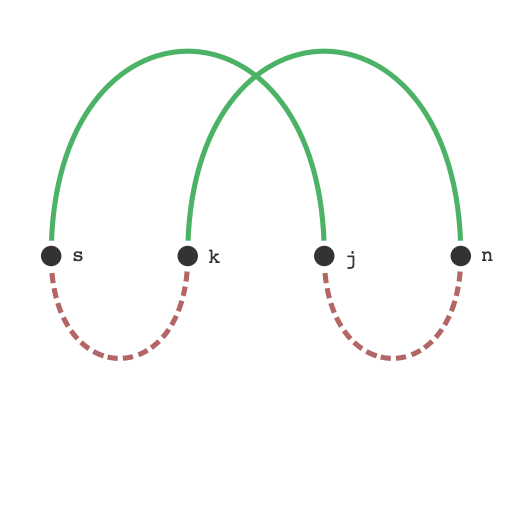
\includegraphics[width=0.3\textwidth]{images/nodes_to_switch_before.png}
        \caption{Wyróżnione wierzchołki i krawędzie między nimi. Linia przerywana oznacza brak krawędzi.}
    \end{figure}
    
    Ale możemy teraz zmienić ,,status'' wyróżnionych krawędzi, tzn. odrzucić krawędzie $v_sv_j$ i~$v_kv_n$ oraz dodać krawędzie $v_sv_k$ i~$v_jv_n$.
    
    \begin{figure}[H]
        \centering
        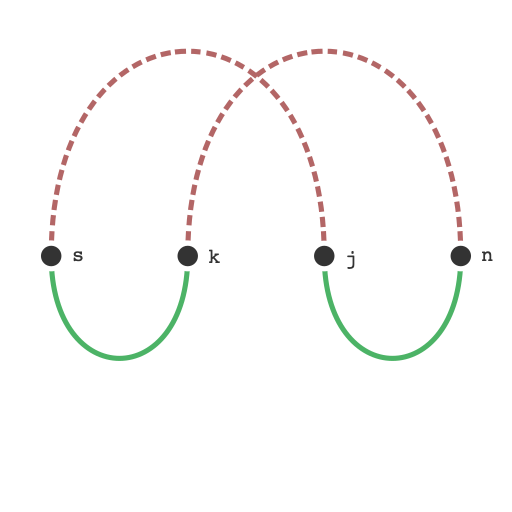
\includegraphics[width=0.3\textwidth]{images/nodes_to_switch_after.png}
        \caption{Wyróżnione wierzchołki po zamianie statusu krawędzi}
    \end{figure}
    
    Zauważmy, że każdy z~wierzchołków, których dotknęła powyższa operacja, stracił jedną krawędź i~zyskał jedną krawędź, więc sekwencja stopni nie uległa zmianie. Załataliśmy natomiast ,,dziurę'' pod indeksem $j$. Mamy zatem graf $G'$, który ma następujące własności:
    \begin{itemize}
        \item $G' \in \mathcal{G}$, ponieważ zgadza się sekwencja grafowa. A~zatem w~$G'$ jest ,,dziura'' wśród $d_n$ wierzchołków bezpośrednio poprzedzających $v_n$
        \item najpóźniejsza dziura znajduje się wcześniej niż pod indeksem $j$, bo tam była w~$G$, a~w~$G'$ została załatana
    \end{itemize}
    Ale przecież wybraliśmy $j$~w~taki sposób, aby było minimalne! Mamy zatem sprzeczność z~wyjściowym założeniem i~dowiedliśmy, że istnieje $G \in \mathcal{G}$ taki, że dla każdego $i \in [n - d_n, n - 1]$ mamy krawędź $v_iv_n$. Możemy zatem odrzucić wierzchołek $v_n$ i~uzyskać w~ten sposób graf, którego sekwencją stopni jest $\pars{d_1', \ldots, d_{n - 1}'}$! A~to właśnie chcieliśmy udowodnić.
  \end{proof}